\section{Evaluation Methodology}

\cut{This section describes the evaluation methodology applied to \SUMMA.}

The \SUMMA evaluation \ins{paradigm} covers different types of evaluation, depending on the aspects or viewpoints – these will be further elaborated upon in the paragraphs below. It will include, for instance, \replace{technically-focused}{tests focused on technology} vs. user-centric evaluation; testing of components vs. the integrated platform; lab vs. field tests; verification vs. validation; \cut{and} formative vs. summative evaluation. \cut{User testing of the prototypes during the agile software design and development phase follows the V-model.}

\subsection{Technical Testing and User-Centered Evaluation}
T\cut{hus, t}he consortium will perform and execute technical testing as well as user-centered evaluation and trials. Technical test\replace{ing}{s} will be \replace{done}{conducted} by the technical partners, on components, technologies, and specific functionalities. These will primarily be reported in the respective technical deliverables of the system. User-centered evaluation emphasises the role of the user rather than the system and considers the needs of the end users. It focuses upon testing the prototype or specific modules in a near-real-life scenario by giving test persons realistic tasks in a staged, yet realistic environment.

\subsection{Components and Integrated Platform/Prototype Testing}
Users will participate in the evaluation of  individual components/technologies. These include, for instance, ASR, machine translation, automated summarisation and clustering. In these tests, the focus is on a particular technology in isolation, limited to specific languages. The focus can be on functionality as well as output quality.

Integrated Platform and Prototype testing is at the integrated level, i.e. the operation of the platform and prototype with all technologies integrated.

%\subsubsection{Verification and Validation (V\&V)}
%\ins{%
%When evaluating technology, it is useful to differentiate between software \textit{verification} and software \textit{validation}.
%\textit{Verification} ensures that the software works as specified; \textit{validation} checks if the software accomplishes what it was built for.
%}% end of insertion

%\cut{%
%``Verification and validation are not the same thing'', although there is often confusion as to the distinction. ``In software project management, software testing, and software engineering, verification and validation (V\&V) is the process of checking that a software system meets specifications and that it fulfills its intended purpose, i.e., software quality control.'' Software verification is ``the responsibility of software testers as part of the software development lifecycle.'' It answers the questions: ``Assuming we should build X, does our software achieve its goals without any bugs or gaps?'' Software validation, on the other hand, is: ``Was X what we should have built? Does X meet the high-level requirements?''}% end of cut; if cut, delete footnote below \footnote{\url{https://en.wikipedia.org/wiki/Software_verification_and_validation}}

%\ins% end of insertion

%The verification of technical components (developed in WP3, WP4, WP5) will be carried out by the technical partners. Some components will  be evaluated by test users in the focus group. The usability evaluation (see Sec.~\ref{sec-user-evaluation}) will validate the \SUMMA platform as a whole to test whether it is fit for purpose.


\subsection{Formative and Summative Testing}
Depending on \cut{the time} when \cut{the} testing \replace{is done}{takes place} and the specific goals of the user evaluation, we can distinguish between \textit{formative} \cut{testing} and \textit{summative} testing.

\textit{Formative testing} is carried out during the development phase and focuses on identifying and fixing problems. This kind of testing will take place within the individual work packages as well as during the user evaluation of the different iterations of the prototype. Formative testing aims to provide developers with insight on how users evaluate a specific status of the prototype within the development cycle. It is less about metrics or statistics, but about finding out what works best for users. The findings from formative testing will feed directly into the development process. \replace{In principle, f}{F}ormative testing \ins{typically} \replace{will be done with}{involves} small focus groups of \ins{at most} 5 people.
This focus group size has been shown to be the most cost-effective for formative testing --- more users do not substantially improve feedback quality~\citep{neilson2000}.
%\footnote{Jakob Nielsen in \url{https://www.nngroup.com/articles/why-you-only-need-to-test-with-5-users}, March 19, 2000.}
% \cut{maximum}\replace{, as i}{. I}t has been proven that more users do not substantially increase feedback quality, provided iterative testing is applied, according to Jakob Nielsen's theory in "Why You Only Need to Test with 5 Users" (March 19, 2000). \footnote{\url{https://www.nngroup.com/articles/why-you-only-need-to-test-with-5-users}} \UG{References? - inserted, but format to be corrected by UEDIN} That number is, therefore, the most cost-effective one.

\textit{Summative testing} validates whether the finished product meets the user requirements. Summative testing is primarily carried out during the evaluation of the final prototype at the end of the project. Summative testing is an ultimate evaluation of the tool in terms of measurable usefulness, efficiency, user-friendliness and satisfaction.

%The distinction between formative and summative testing is relevant to the scope of the evaluation. Formative testing aims to provide developers with insight on how users evaluate a specific status of the prototype within the development cycle. It is less about metrics or statistics, but about finding out what works best for users. The findings from formative testing will feed directly into the development process. Summative testing is an ultimate evaluation of the tool in terms of measurable usefulness, efficiency, user-friendliness and satisfaction. Summative testing, on the other hand, may involve a larger number of users. 

%\replace{In principle, f}{F}ormative testing \ins{typically} \replace{will be done with}{involves} small focus groups of \ins{at most} 5 people \cut{maximum}\replace{, as i}{. I}t has been proven that more users do not substantially increase feedback quality, provided iterative testing is applied, according to Jakob Nielsen's theory in "Why You Only Need to Test with 5 Users" (March 19, 2000). \footnote{\url{https://www.nngroup.com/articles/why-you-only-need-to-test-with-5-users}} \UG{References?} That number is, therefore, the most cost-effective one. Summative testing, on the other hand, may involve a larger number of users.

\subsection{Lab and Field Trials}

\textit{Lab trials} These are trials with small numbers of users with limited features and content sets potentially on site at Deutsche Welle and BBC Monitoring. They are organised in the form of focus group testing. The users for such trials will not be on duty at the time, and although the content may be as live and they may be acting through their full workflow, this will not be in the actual operational team. These trials are common to the most in-depth and intensive testing phases of the agile prototyping cycles. These tests involve both platform testing and application/use case testing. 

\textit{Field trials} These trials are a step beyond the main prototyping cycle of development and testing. With the field trials, integrated and tested user interfaces will be tested and trialed with real users in the actual working environment for limited periods of time. Field trials may be limited in functionality, languages, research subjects/areas or content types. Field trials will be an opportunity to assess the impact of the new tools on the larger workflow and operation. These evaluation sessions will be started as early as possible within the project. Depending on the user scenario and language coverage, such experimental field trials will include up to 15 participants, including journalists, editors, monitors, and analysts – the exact number of journalists evolves with the prototyping process and will be defined together with the operational management. All available and regularly covered media streams and content sources, processable by the \SUMMA system will potentially be included.

\subsection{V-Model of Evaluation}\label{sec-vmodel}
\SUMMA uses the V-Model as its primary model for its evaluation activities. 
%\UG{Insert a reference to the figure here. done}
%
%\UG{An brief explanation of the waterfall model would be in order here. I assume the explanation below explains it.}
%
\cut{As explained in }Wikipedia%
\replace{,}{\ explains it as follows}: ``In software development, the V-model represents a development process that may be considered an extension of the waterfall model. Instead of moving down in a linear way, the process steps are bent upwards after the coding phase, to form the typical V shape. The V-Model demonstrates the relationships between each phase of the development life cycle and its associated phase of testing. The horizontal and vertical axes represent time or project completeness (left-to-right) and level of abstraction (coarse or grain abstraction), respectively.''\footnote{\url{https://en.wikipedia.org/wiki/V-Model_(software_development)}}
Figure \ref{fig:V-Model} below visualises the model.

The major purpose of the V-Model is to meet business requirements and enhance confidence in the tool or application. It supports testing in early stages of the development process. Each verification level has a validation counterpart. 

The left side outlines the project definition/development phases, while the right side shows user-centric project test and evaluation. At the bottom, code relates to the implementation phase.

The figure below shows the occurrence of the verification and validation processes. 

\begin{figure}[ht]
    \centering
    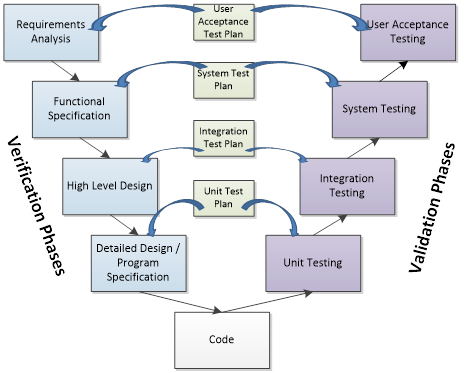
\includegraphics[width=1.0\textwidth]{./images/V-Model.png}
    \caption{V-Model for Evaluation}
    \label{fig:V-Model}
\end{figure}


\subsection{User Evaluation phases}
In the V-model, each stage of the technical testing has a corresponding stage for user evaluation. The following are the typical phases of user evaluation in the V-Model. 

\paragraph{Unit testing}
\cut{In the V-Model, }Unit Test Plans (UTPs) are developed during module design phase. These UTPs are executed to eliminate bugs at code level or unit level. A unit is the smallest entity which can independently exist, e.g. a program module. Unit testing verifies that the smallest entity can function correctly when isolated from the rest of the codes/units. In \SUMMA this will relate to component and technology testing.

\paragraph{Integration testing}
Integration Test Plans are developed during the Architectural Design Phase. These tests verify that units created and tested independently can coexist and communicate in the integrated platform. In \SUMMA, integration testing is performed primarily by the integrator partner LETA, although user partners will also run tests on the integrated platform, regardless of the UI status, at request. 

\paragraph{System testing}
System Tests Plans are developed during System Design Phase. The whole application is tested for its functionality, interdependency and communication. It tests whether the system works as it is intended to work. In \SUMMA, this refers to functionality testing of the system by the user partners.

\paragraph{User acceptance testing}
User Acceptance Test (UAT) Plans are developed during the Requirements Analysis phase. UAT is performed in a user environment that resembles the production environment, using realistic data. UAT verifies that delivered system meets user requirements and that the system is ready for use in real time. In \SUMMA this constitutes user testing for the benefit of the agile prototyping team. 

As Figure~\ref{fig:V-Model} above shows, the two streams are \cut{in} parallel. Each of the technical work packages will carry out verification of the technical deliverables (their respective technical components). Test users will validate the usability of the platform as well as test the functionality of the system during the design phase.
